%From https://egu2018.eu/PICO_how-to_guide_to_PICO.pdf
%Abstracted and templated by Brian Ballsun-Stanton, Macquarie University.
%original template by https://github.com/snowtechblog/pico-latex-presentation by Anselm Köhler

\documentclass[unknownkeysallowed,usepdftitle=false, parskip=full]{beamer}
% unknownkeysallowed is needed for mac and the newer latex version -> is more picky than before...
\usetheme[headheight=1cm,footheight=2cm]{boxes}
%\usetheme{default}


\usepackage{default}
\usepackage{graphicx}
%example pictures created via: http://lorempixel.com/1200/800/cats/Figure2/. Credit to http://lorempixel.com/images.php

\usepackage{epsfig}
\usepackage{siunitx}
\usepackage{color}
\usepackage{ifthen}
%usepackage{ragged2e}

\usepackage[T1]{fontenc}
\usepackage[utf8]{inputenc}
%https://tex.stackexchange.com/a/203804/5483

\usepackage[activate={true,nocompatibility},final,tracking=true,kerning=true,spacing=true,factor=1100,stretch=10,shrink=10]{microtype} % http://www.khirevich.com/latex/microtype/
\microtypecontext{spacing=nonfrench}

\usepackage{lipsum} % for dummy text only
\usepackage[UKenglish]{babel} %https://tex.stackexchange.com/a/27743 
\usepackage[pangram]{blindtext} % https://tex.stackexchange.com/a/48411

%\usepackage{parskip} % from https://tex.stackexchange.com/q/11622
%\setlength{\parskip}{12pt} 

%\setparsizes{\parindent}{12pt}{\parfillskip}

%\usepackage{etoolbox} % as per https://tex.stackexchange.com/a/24331
%\appto\chapterheadendvskip{\vspace{-1\parskip}}
%\setparsizes{\parindent}{50pt plus 20pt minus 30pt}{\parfillskip}

\setbeamertemplate{navigation symbols}{}%remove navigation symbols
\setbeamersize{text margin left=1cm,text margin right=1cm}

% some colors
\definecolor{grau}{gray}{.5}
\definecolor{slfcolor}{rgb}{0,0.6274,0.8353}
\definecolor{wslcolor}{rgb}{0,0.4,0.4}

% setup links
\hypersetup{%
	%linkbordercolor=green,%
	colorlinks=false,%
	pdfborderstyle={/S/U/W 0},%
	%pdfpagemode=FullScreen,%
	pdfstartpage=4%
	}

% setup some fonts
\setbeamerfont{title}{series=\bfseries, size=\small}
\setbeamerfont{author}{size*={5pt}{0pt}}
\setbeamerfont{institute}{size*={3pt}{0pt}}
\setbeamerfont{bodytext}{size=\scriptsize}
	
% Title setup	
\title{Discourse network twitter for rtweet}
\author{Roslyn Walker, Macquarie University, Sydney\inst{}  \and \inst{} \and\inst{}}
\institute{\inst{}
\quad \inst{}}
% add title in headbox
\setbeamertemplate{headline}
{\leavevmode
\begin{beamercolorbox}[width=1\paperwidth]{head title}
  % LOGO
  \begin{columns}[t, totalwidth=\textwidth]
  \begin{column}[c]{1.05cm}
     \includegraphics[width=1cm]{children.png
     }
  \end{column}
  % TITLE
   \begin{column}[c]{10.6cm}
   \centering \usebeamerfont{title} \textcolor{slfcolor}{\inserttitle} \\
   \centering \usebeamerfont{author} \color[rgb]{0,0,0} \insertauthor \\
   \vspace{-0.05cm}
   \centering \usebeamerfont{institute} \insertinstitute
  \end{column}
  % PICTURE
  \begin{column}[c]{1.15cm}
    \hspace{0.005cm}
    \includegraphics[width=1cm]{figure/children.png}
  \end{column}
  \end{columns}
  {\color{slfcolor}\hrule height 1pt\vspace{0.1cm}}
\end{beamercolorbox}%
}

% setup the navigation in footbox
% first set some button colors
\newcommand{\buttonactive}{\setbeamercolor{button}{bg=wslcolor,fg=white}}
\newcommand{\buttonpassive}{\setbeamercolor{button}{bg=slfcolor,fg=black}}
% now set up that the one active one gets the new color.
\newcommand{\secvariable}{nothing}
% therefore we write before each section (well, everything which should be part of the navi bar)
% the variable \secvariable to any name which is in the next function ...
\newcommand{\mysection}[1]{\renewcommand{\secvariable}{#1}
}
% ... compaired to strings in the following navibar definition ...
\newcommand{\tocbuttoncolor}[1]{%
 \ifthenelse{\equal{\secvariable}{#1}}{%
    \buttonactive}{%
    \buttonpassive}
 }
% ... here we start to set up the navibar. each entry is calling first the function \tocbuttoncolor with the argument which should be tested for beeing active. if active, then change color. afterwards the button is draw. so to change that, you need to change the argument in \toc..color, the first in \hyperlink and before each frames definition... A bit messed up, but works...
\newlength{\buttonspacingfootline}
\setlength{\buttonspacingfootline}{-0.2cm}
\setbeamertemplate{footline}
{\leavevmode
\begin{beamercolorbox}[width=1\paperwidth]{head title}
  {\color{slfcolor}\hrule height 1pt}
  \vspace{0.05cm}
  % set up the buttons in an mbox
  \centering \mbox{
    \tocbuttoncolor{abstract}
    \hyperlink{abstract}{\beamerbutton{2 Minute Madness}}
    \tocbuttoncolor{radar}
    \hspace{\buttonspacingfootline}
      \hyperlink{radar}{\beamerbutton{Section 1}}

    \tocbuttoncolor{line}
    \hspace{\buttonspacingfootline}
      \hyperlink{line}{\beamerbutton{Section 2}}
    \tocbuttoncolor{major}
    \hspace{\buttonspacingfootline}
      \hyperlink{major}{\beamerbutton{Section 3}}
    \tocbuttoncolor{slab}
    \hspace{\buttonspacingfootline}
      \hyperlink{slab}{\beamerbutton{Section 4}}
    \tocbuttoncolor{minor}
    \hspace{\buttonspacingfootline}
      \hyperlink{minor}{\beamerbutton{Section 5}}
    \tocbuttoncolor{conclusion}
    \hspace{\buttonspacingfootline}
      \hyperlink{conclusion}{\beamerbutton{Conclusion}}
    % this last one should normaly not be used... it will open the preferences to change the 
    % behaviour of the acrobat reader in fullscreen -> usefull in pico...
    \setbeamercolor{button}{bg=white,fg=black}
    % for presentation
    %\hspace{-0.1cm}\Acrobatmenu{FullScreenPrefs}{\beamerbutton{\#}}
    % for upload
    
     
\Acrobatmenu{FullScreenPrefs}{\vspace{0.3cm}\hspace{0.24cm}\mbox{%
      
\includegraphics[height=0.04\textheight,keepaspectratio]{%
	  figure/CreativeCommons_Attribution_License.eps}%
	  }}
   }
    \vspace{0.05cm}
\end{beamercolorbox}%
}


\begin{document}


%%%%%%%%%%%%%%%%%%%%%%%%%%%%%%%%%%%%%%%%%%%%%%%%%%%%%%%%%%%%%%%%%%%%%%%%%%
\mysection{abstract}
%%%%%%%%%%%%%%%%%%%%%%%%%%%%%%%%%%%%%%%%%%%%%%%%%%%%%%%%%%%%%%%%%%%%%%%%%%
\begin{frame}\label{\secvariable}

\usebeamerfont{bodytext}


\parbox{\linewidth}{

Collins Dictionary named Climate Strike the word of 2019:


\vspace{12pt}

"a form of protest in which people absent themselves from education or work in order to join demonstrations demanding action to counter climate change"

 \vspace{12pt}
 
"Climate Strike and public discourse" is the topic of my thesis.

 \vspace{12pt}
 
 In my research I've encountered two issues with gathering empirical data from public discourses around Climate Strike.

\vspace{12pt}
(1) Ethical considerations for collecting data from social media.

\vspace{12pt}
(2) How do I validate the hashtag public "ClimateStrike" on Twitter as a global conversation?

\vspace{12pt}
As a solution I've written an R script to scrape Twitter.





 \vspace{12pt}
 
%Praesent dolor nibh, malesuada quis convallis sit amet, volutpat at purus. Suspendisse sed velit quis turpis venenatis fermentum ut sed tellus. Ut eu lacus ultricies, elementum ex gravida, gravida elit. Donec gravida nisl sit amet nulla vestibulum, in malesuada diam varius. Donec sodales efficitur nulla, non tincidunt nibh commodo nec. 
}


   
\end{frame}



\begin{frame}\label{\secvariable}
  \begin{columns}[t]
  %https://tex.stackexchange.com/a/7452/5483
  \begin{column}[c]{0.40\textwidth}

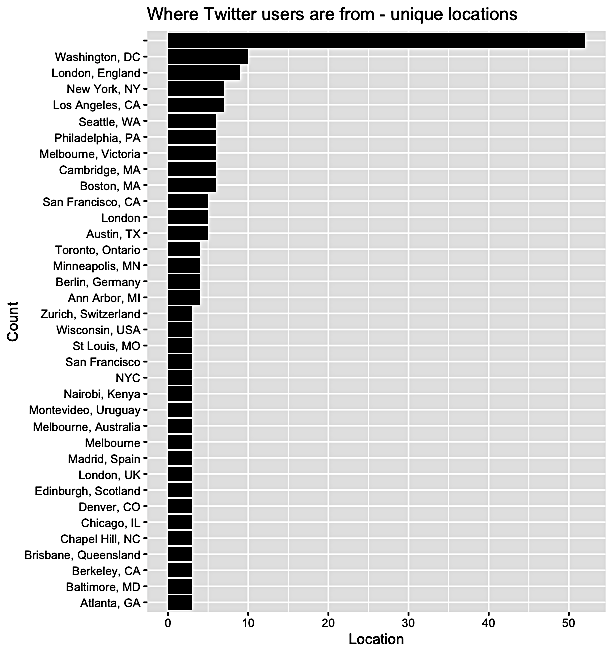
\includegraphics[width=2\textwidth,height=4\textheight,keepaspectratio]{%
figure/Rplot01.png}
    \end{column}
    \begin{column}[c]{0.45\textwidth}
    \parbox{\linewidth}{

      The output  is a chart that aggregates the location of people using the term ClimateStrike.
      
      
 \vspace{12pt}

The distribution of the public users on Twitter by geolocation without accessing their private information or identity. 

      }
    \end{column}
    
  \end{columns}

  
\end{frame}

%%%%%%%%%%%%%%%%%%%%%%%%%%%%%%%%%%%%%%%%%%%%%%%%%%%%%%%%%%%%%%%%%%%%%%%%%%
\mysection{radar}
%%%%%%%%%%%%%%%%%%%%%%%%%%%%%%%%%%%%%%%%%%%%%%%%%%%%%%%%%%%%%%%%%%%%%%%%%%
\begin{frame}\label{\secvariable}
  \begin{columns}[t]
  %https://tex.stackexchange.com/a/7452/5483
    \begin{column}[c]{0.45\textwidth}
    \parbox{\linewidth}{

    Social media data is a valuable research source for a critical discourse analysis.
       \vspace{12pt}
       
Sensitivity considerations for collecting data from social media platforms. 
 \vspace{12pt}
 
Data reflects the political opinions of the contributors their identity may be discovered through an online search.
 \vspace{12pt}

      }
    \end{column}
    \begin{column}[c]{0.45\textwidth}
%http://lorempixel.com/1200/800/cats/children/     
%http://lorempixel.com/1200/800/cats/children/
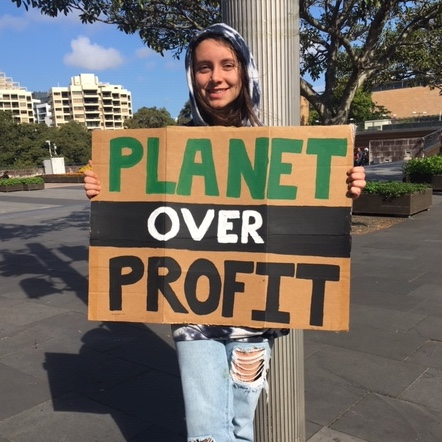
\includegraphics[width=1\textwidth,height=0.5\textheight,keepaspectratio]{%
figure/girl.png}\\
\vspace{12pt}
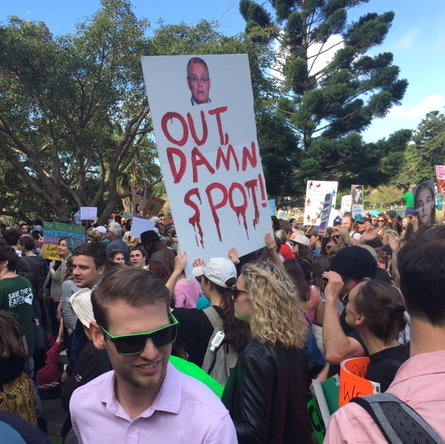
\includegraphics[width=1\textwidth,height=0.5\textheight,keepaspectratio]{%
figure/spot.png}
    \end{column}
  \end{columns}

  
\end{frame}

%%%%%%%%%%%%%%%%%%%%%%%%%%%%%%%%%%%%%%%%%%%%%%%%%%%%%%%%%%%%%%%%%%%%%%%%%%
\mysection{line}
%%%%%%%%%%%%%%%%%%%%%%%%%%%%%%%%%%%%%%%%%%%%%%%%%%%%%%%%%%%%%%%%%%%%%%%%%%
\begin{frame}\label{\secvariable}
\begin{center}
  \vspace{-0.5cm}
  %http://lorempixel.com/1200/800/cats/Figure4/
 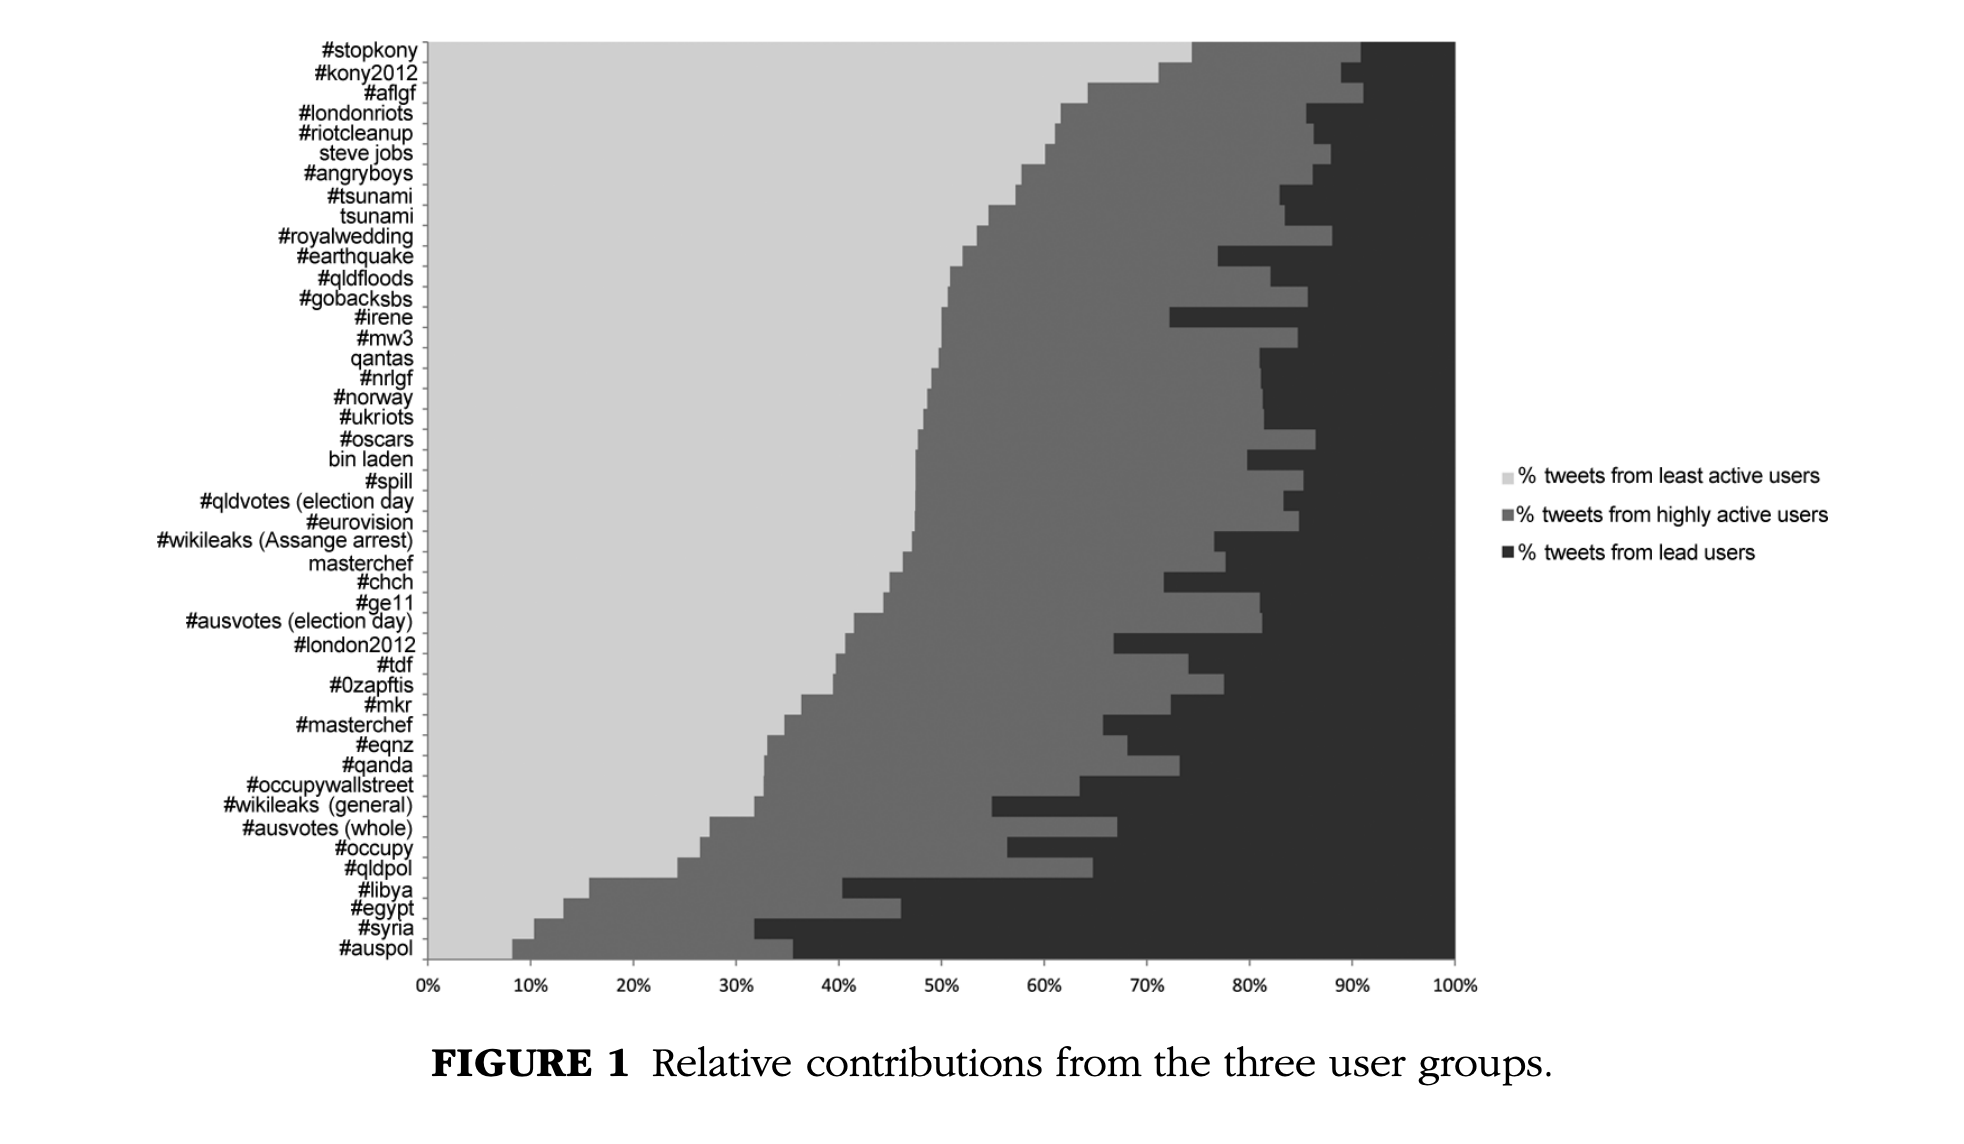
\includegraphics[width=1.1\textwidth,height=1\textheight,keepaspectratio]{%
  figure/user_group.png}
\end{center}
  \vspace{-0.5cm}
  \begin{enumerate}[]
  
  
\item
  \end{enumerate}
\usebeamerfont{bodytext} 
  $\quad \Rightarrow$  Image source: reproduced from Bruns and Steiglitz (2012: 171). Twitter activity patterns among user groups.
  
\end{frame}

%%%%%%%%%%%%%%%%%%%%%%%%%%%%%%%%%%%%%%%%%%%%%%%%%%%%%%%%%%%%%%%%%%%%%%%%%%
\mysection{major}
%%%%%%%%%%%%%%%%%%%%%%%%%%%%%%%%%%%%%%%%%%%%%%%%%%%%%%%%%%%%%%%%%%%%%%%%%%
\begin{frame}\label{\secvariable} %%Eine Folie
\begin{center}
%http://lorempixel.com/1200/800/cats/Figure5/
 \includegraphics[width=1\textwidth,height=0.75\textheight,keepaspectratio]{%
  figure/rstudio.png}
\end{center}

    \parbox{\linewidth}{

My research uses rtweet in Rstudio to gather communicative actions within a hashtag community. This informs the information flow around an issue within and among communities.
}
\end{frame}

%%%%%%%%%%%%%%%%%%%%%%%%%%%%%%%%%%%%%%%%%%%%%%%%%%%%%%%%%%%%%%%%%%%%%%%%%%
\mysection{slab}
%%%%%%%%%%%%%%%%%%%%%%%%%%%%%%%%%%%%%%%%%%%%%%%%%%%%%%%%%%%%%%%%%%%%%%%%%%
\begin{frame}\label{\secvariable}
%http://lorempixel.com/1200/800/cats/Figure6/
\begin{center}

\includegraphics[width=0.50\textwidth,height=0.50\textheight,keepaspectratio]{%
figure/howgood.png}
\end{center}
    \parbox{\linewidth}
    {

I use Twitter as the digital technology for my research due to public status of tweets which are by default public.
My study considers the affordance of digital technologies, such as Twitter, for civic protest for social change.
}

\hyperlink{slabtable}{\beamerbutton{more \dots}}


\end{frame}



\begin{frame}\label{slabtable}
\begin{columns}
\begin{column}[t]{1.1\textwidth}
\hyperlink{slab}{\beamerbutton{\dots }}\\
%Morbi mauris turpis, ornare eu elit quis, pulvinar bibendum sapien. Nulla vel justo id dui aliquam blandit. Etiam pellentesque ac nisl ut suscipit. 

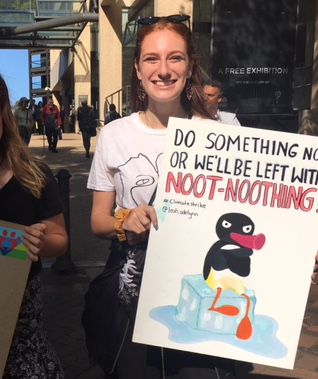
\includegraphics[width=0.30\textwidth,height=0.30\textheight,keepaspectratio]{%
figure/dosomething.png}

This proof of concept has three main goals:
\usebeamerfont{bodytext} 
\item 
(1) send request to Twitter's stream APIs
\item 
(2) retrieve data
\item 
(1) format data into a structure 
\item 
As a social media researcher, I wanted to access public social media postings as data, so that I could analyse the data collected under a hashtag public and identify discourse circulation patterns. As a social media researcher, I wanted to extract tweets based on a hashtag through metadata (place).


\vspace{0.3cm}
\end{column}
\end{columns}
 

\end{frame}




%%%%%%%%%%%%%%%%%%%%%%%%%%%%%%%%%%%%%%%%%%%%%%%%%%%%%%%%%%%%%%%%%%%%%%%%%%
\mysection{minor}
%%%%%%%%%%%%%%%%%%%%%%%%%%%%%%%%%%%%%%%%%%%%%%%%%%%%%%%%%%%%%%%%%%%%%%%%%%
\begin{frame}\label{\secvariable} %%Eine Folie
\begin{center}
%http://lorempixel.com/1200/800/cats/Figure7/
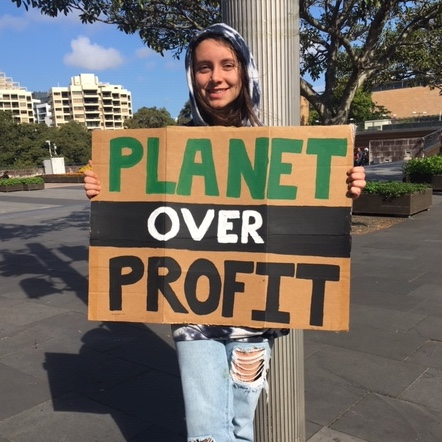
\includegraphics[width=0.5\textwidth,height=0.5\textheight,keepaspectratio]{%
figure/girl.png}
\end{center}
\vspace{-0.2cm}

Quality assurance
\usebeamerfont{bodytext} 
\item The acceptance tests for this proof of concept includes whether the data retrieved is in an accessible format that enables the exporting, sorting, collecting, analysis, and archiving of the data output. 
\item 
The acceptance criteria includes the use of automated tools to access and manipulate the data output.
\item 
These acceptances have been met by this proof of concept.


\end{frame}

%%%%%%%%%%%%%%%%%%%%%%%%%%%%%%%%%%%%%%%%%%%%%%%%%%%%%%%%%%%%%%%%%%%%%%%%%%

%%%%%%%%%%%%%%%%%%%%%%%%%%%%%%%%%%%%%%%%%%%%%%%%%%%%%%%%%%%%%%%%%%%%%%%%%%
\begin{frame}\label{\secvariable}

%
\includegraphics[width=0.45\textwidth,height=0.25\textheight,keepaspectratio]{%
figure/children.png}\hspace{.05\textwidth}

Limitations of the proof of concept
\usebeamerfont{bodytext} 
\item 
(1) Access to data on Twitter requires a personal application programming interface (API) key. Source: https://developer.twitter.com/en/apps
\item 
(2) Before using this software a user requires a secret pair for the OAuth flow.
\item 
(3) The process of accessing Twitter changes frequently, so that software written to interact with the Twitter client requires frequent testing and revision.
\item 
(4) None of the four private pieces of identity and authentication information should ever be committed to public source control, in order to protect your application and/or user account from compromise or misuse.
Source: https://twittercommunity.com/t/upcoming-changes-to-access-token-and-secret-management/130851


\end{frame}

%%%%%%%%%%%%%%%%%%%%%%%%%%%%%%%%%%%%%%%%%%%%%%%%%%%%%%%%%%%%%%%%%%%%%%%%%%
\mysection{conclusion}
%%%%%%%%%%%%%%%%%%%%%%%%%%%%%%%%%%%%%%%%%%%%%%%%%%%%%%%%%%%%%%%%%%%%%%%%%%
\begin{frame}\label{\secvariable}
  

References:

\vspace{12pt}
\usebeamerfont{bodytext} 
\item Bruns, A. (2018a) "Digital Public Spheres in Australia"  in  Digitizing Democracy, Routledge
\item 
  
 Bruns, A. and S. Stieglitz (2012) Quantitative Approaches to Comparing Communication Patterns on Twitter, Journal of Technology in Human Services % Image source: reproduced from Bruns and Steiglitz (2012: 171). Twitter activity patterns among user groups.
\item 
Elster Hanson, J. (2019) ‘Climate strike’ named 2019 word of the year by Collins Dictionary' in The Guardian, 7 November 2019
\item 

Henderson-Sellers, A. (2010) "How seriously are we taking climate change? Monitoring climate change communication," Sydney: Sydney University Press.

\item 

Pew Center Research (2019) "A look at how people around the world view climate change" from the  Pew Research Center’s Spring 2018 Global Attitudes Survey.

\item 
Pico Presentation: https://github.com/MQ-FOAR705/Walker_Roslyn_PICO_Presentation

%  \item Quisque sed orci eu libero mattis lobortis. Curabitur aliquam lorem neque, ac auctor justo sagittis sed. Nunc augue nisl, mattis sed turpis at, elementum lobortis augue. Vestibulum porta felis bibendum mattis iaculis. Nulla dignissim varius rutrum.
%  \item Vivamus eget semper nunc. Donec sodales ornare porttitor. Curabitur commodo viverra arcu. Aliquam consequat felis non dolor consequat ultricies. Mauris non finibus nisl. Sed tincidunt felis at porttitor posuere.

\end{frame}

\end{document}
